\cotefile{82}
\scanpage{32}
encore que $E'$ opère \uline{\unsure{fidèlt|fidèlmt}} sur $E$ par $\rho_E\deleted{\unsure{'}}$, quand \deleted{\unsure{on}} $S=\operatorname{Spec}k$, $k$ corps alg. clos. Or dans ce cas on peut trouver une base $e_1,e_2,e_3$ p.r. à laquelle $q$ se met sous la forme $xy+z^2$, $\omega=e_1\wedge e_2\wedge e_3$ (quitte \inserted{au besoin} à changer $e_3$ en $-e_3$\ldots) et il suffit de prendre alors les calculs de (72)
\[
\rho_E(xX+hH+yY):
\left\{\begin{aligned}
\widetilde X&\longmapsto h\widetilde X-y\widetilde H\\
\widetilde Y&\unsure{\vdash|\longmapsto} x\widetilde H\unsure{=|-|+}h\widetilde Y\\
\widetilde H&\longmapsto-2x\widetilde X+2y\widetilde Y\deleted{\unsure{+}}
\end{aligned}\right.
\]
\[
\rho_E(xX+hH+yY)=0\quad\Longrightarrow x=y=h=0\qquad\text{o.k.}
\]

Il faut encore définir l'isom.
\[
 E\xrightarrow{\sim}\unsure{\mathfrak g|\mathfrak g'|\widetilde{\mathfrak g}}
\]
et prouver ses propriétés. Pour ceci, il faut redéfinir ou préciser, en termes élémentaires, la construction de $\widetilde G$ sur $G$ -- il nous faut pour ceci ouvrir une parenthèse
% archive sheet number: 31
\scanpage{34}
% archive sheet number: 33
\[
\begin{aligned}
F_3&=T\\
F_4&=T-1\\
F_5&=T^2-T-1\\
F_6&=T-2
\end{aligned}
\]
On peut définir $F_n$ comme le polynôme minimal (sur $\mathbb Q$) de $1+2\cos 2\pi/n$, \deleted{\unsure{de $1+$}} ou encore de $1+\zeta+\zeta^{-1}$, où $\zeta$ est une racine \uline{primitive} $n$.ième de l'unité.

\noindent\rule{.88\linewidth}{.3pt}
\diagram{\begin{tikzcd}[ampersand replacement=\&,column sep=small]
\zeta_0\arrow[r,"\underbrace{\hspace{1.4em}}_{e_1}"']\& \zeta_1\&\zeta_2\&\zeta_3
\end{tikzcd}}
\[
\begin{aligned}
\zeta_1-\zeta_0&=e_1\\
\zeta_2\unsure{-|\cdot}\zeta_1&=e_2
\end{aligned}
\qquad
\left\{\begin{aligned}
u(\zeta_0)&=\zeta_0+e_1\\
u(e_1)&=\zeta_2-\zeta_1=e_2\\
u(e_2)&=\zeta_3-\zeta_2=-e_1+(\alpha-1)e_2
\end{aligned}\right.
\]
\figure{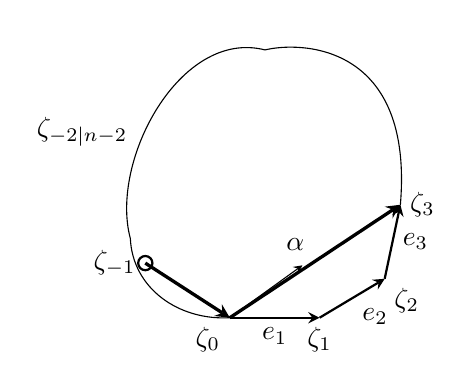
\begin{tikzpicture}[scale=.95,>=stealth]
\coordinate (a) at (-1.65,-.72);
\coordinate (b) at (-.52,-1.45);
\coordinate (c) at (.68,-1.45);
\coordinate (d) at (1.55,-.93);
\coordinate (e) at (1.76,.06);
\draw (e) .. controls (1.94,2.2) and (.45,2.25) .. (-.05,2.13)
 .. controls (-1.18,2.42) and (-2.13,.65) .. (-1.85,-.39)
 .. controls (-1.82,-1.06) and (-1.2,-1.49) .. (b);
\draw[thick] (a) circle (.095);
\draw[->,very thick] (a)--(b);
\draw[->,thick] (b)--node[below]{$e_1$}(c);
\draw[->,thick] (c)--node[below right]{$e_2$}(d);
\draw[->,thick] (d)--node[right]{$e_3$}(e);
\draw[->,very thick] (b)--node[above left]{$\alpha$}(e);
\draw[->] (b)--(.45,-.75);
\node[left] at (-1.76,1.03){$\zeta_{\unsure{-2|n-2}}$};
\node[left] at (a){$\zeta_{-1}$};
\node[below left] at (b){$\zeta_0$};
\node[below] at (c){$\zeta_1$};
\node[below right] at (d){$\zeta_2$};
\node[right] at (e){$\zeta_3$};
\end{tikzpicture}}
\scanpage{35}
\[
\underset{\unsure{\chi|?|\mathfrak g}}{\text{\unsure{Algèbres|Algèbre|Alg Spéc}}}\ (\mathcal M)
\ \unsure{\subseteq|\simeq}\mathbb P(\widetilde{\unsure{M|J|\mathfrak g}})
\simeq \mathbb P^\vee(M)\simeq
\bigl[\check P=\mathrm{Dr}(P)\bigr]\simeq \operatorname{Div}^{+}_{2}(X)
\]
% Note below the second projective-space expression, joined to it by an inclusion sign.
\[
\rotatebox{90}{$\supset$}
\]
\begin{center}
Ss-gpes lisses\\
connexes \unsure{comm.|commut.}\\
\deleted{\unsure{de}} de dim 1\\
dans $G$\\[2pt]
$\unsure{\operatorname{Jac}|J^{\cdot\cdot}|\mathcal T\in\cdots}(G)$
\end{center}

$\operatorname{Cent}(J)=J$ -- le centralisateur de \deleted{\unsure{tte}} \unsure{tte|toute} section de $J$ telle que $g^2\ne1$ en chaque fibre est $J$.

$U=X-Y$ torseur sous $J$

% slanted
\margin{\deleted{\illegible{1}} \unsure{si|en} \unsure{caractér.} \unsure{ou|en} car 2, $\unsure{J_s\simeq\mathbf G_{a,s}|J_s\simeq\mathrm{Ga}_s}$}

\deleted{Dans} $N(J)/J\subset\underline{\operatorname{Aut}}(J)$ \deleted{il y a} la section $\sigma=-\mathrm{id}_J$ est dans $N(J)/J$

\deleted{Soit} \deleted{La} l'image inverse $\unsure{\bar J|\bar{\jmath}|\overline{\mathcal T}}$ de $\sigma$ dans $N(J)$ \deleted{\unsure{est un}} \inserted{qui est un} \deleted{$J$-torseur} $J$-torseur \deleted{$X-Y$, en est une} est comme $X-Y$. \deleted{\unsure{On a}} \deleted{\unsure{c}} \deleted{section ce qui}
\[
\begin{aligned}
(X-Y)&\longrightarrow\bar J\\
J&\xrightarrow{2\,\mathrm{id}_J} J
\end{aligned}
\]
% archive sheet number: 34
\scanpage{37}
Soit\deleted{\unsure{ent|es}} $S$ schéma, \deleted{$u\in M_2(S)=M_2(\Gamma(S,\mathcal O_S))$, supposons} \inserted{$V$ \deleted{fibré} \inserted{Module} vectoriel de rang 2, $u\in\operatorname{End}(V)$}
\[
 \forall s\in S,\qquad u_s\notin k(s).1 \tag*{(1)\deleted{\unsure{'}}}
\]
Considérons le commutant de $u$ dans $\underline{\operatorname{End}}(V)$ (le foncteur). Je dis qu'il est égal au sous-fibré vectoriel $\mathcal O_S\,\mathrm{Id}+\mathcal O_S\,u$ de $\underline{\operatorname{End}}(V)$ -- donc le commutant dans $\operatorname{GL}(V)$ est formé des $\alpha\,\mathrm{id}+\beta u$, avec
\[
 \det(\alpha\,\mathrm{id}+\beta u)=\alpha^2+\alpha\beta\operatorname{Tr}u+\beta^2\det u\ \deleted{\unsure{\ne}}\quad\text{inv.} \tag*{(2)}
\]
donc le commutant (ou stabilisateur) dans $\underline{\operatorname{GP}}(V)$ s'identifie au
\[
 C_{\underline{\operatorname{GP}}(V)}(u)\simeq\mathbb P^1-Q_{\operatorname{Tr}u,\det u}
\]
où $Q_{\deleted{\unsure{\operatorname{Tr}u}}\tau,\delta}$ désigne, de façon \unsure{général|générale}, la ``\unsure{0-|o-}quadrique'' de $\mathbb P^1$ définie par l'équation quadratique en $\alpha,\beta$
\[
 \alpha^2+\tau.\alpha\beta+\delta.\beta^2\deleted{\det u}
\]
En l'occurrence, c'est un diviseur de degré 2 \deleted{\unsure{donc}} qui est étale sss
\[
 \tau^2-4\delta\qquad\text{inv.}
\]
ce qui, dans le cas $\tau=\operatorname{Tr}u\deleted{\unsure{=0}},\delta=\det u$, signifie que les val. propres de $u$ fibre par fibre sont distinctes,
% archive sheet number: 36
\scanpage{38}
Le sous-groupe \inserted{$H\subset\underline{\operatorname{GP}}(V)$} bien sûr ne dépend que du sous-Module $\unsure{\mathcal O_S|\mathcal O_S1}+\mathcal O_Su$ de $\underline{\operatorname{End}}(V)$, ou ce qui revient au $=$, de son image dans $\underline{\operatorname{End}}(V)/\underline{\mathcal O}_S.1=\underline{\operatorname{Lie}}\,\underline{\operatorname{GP}}(V)$ laquelle image est un sous-fibré inversible qui n'est autre que $\operatorname{Lie}H$. Ceci précise relation entre sous-fibrés vectoriels \inserted{$\mathfrak h$} de rang 1 de $\mathfrak g=\underline{\operatorname{GP}}(V)=G$ et sous-gpes lisses \inserted{connexes et comm. $H$} de \deleted{rang} \inserted{dim rel.} 1 de $\unsure{G|\mathfrak g}$.

Est-il vrai que $H$ est le centralisateur de $\mathfrak h$ \inserted{$=\operatorname{Lie}\unsure{\mathfrak h|H}$}, ou de tte section de $H$ partout $\ne$ section unité, ? à fortiori de $H$ lui-$=$ ?
\[
\begin{aligned}
ghg^{-1}\deleted{\unsure{\ne}}&=\lambda h
& \text{sps }\ \deleted{\unsure{u\ \mathrm{univ.}|\mathrm{unipotent}}}\,\inserted{\det u=-1}\\
\det h&=\lambda^2\det h & \boxed{\lambda^2=1}\\
\deleted{\operatorname{Tr}u}&\deleted{=\lambda\operatorname{Tr}u}
\end{aligned}
\]
\deleted{en car. $\ne2$ on déduit $\lambda=\pm1$ loc$^{\mathrm{t}}$, le cas $+1$ déjà traité, reste \inserted{alors} le cas}
\[
 \deleted{gug^{-1}=-u}
\]
\deleted{Ceci \unsure{est un} n'est possible que si \deleted{les valeurs} \inserted{$\operatorname{Tr}u=0$, donc} (avec $\det u=-1$) est donc \inserted{$u$ une réflexion} \deleted{propres de $u$ sont de la forme} $\{1,-1\}$ (donc distinctes, \deleted{\unsure{et si elles sont}} \inserted{puisqu'elles sont} non nulles), $=$ est conjugué \unsure{à une|une} réflexion dans $G$ donc $u^2=1$} Si on est en car rés. 2,
% archive sheet number: 37
\scanpage{39}
\deleted{\unsure{est un schéma, du moins|est un schéma du fait}} alors un \unsure{ss-groupe|u-groupe|s.-groupe} étale \deleted{qui en chaque fibre est : \unsure{or on} a la condition de \unsure{rang 2 des fibres}} -- donc il s'identifie à un sous-groupe ouvert \deleted{et fermé} de $(\mathbb Z/p\mathbb Z)^*_S$, qui coïncide avec le sous-groupe ouvert $\{\pm1\}$ fibre par fibre, donc \inserted{lui} est égal.

La condition de normalisation \inserted{sur une section $\bar g\in\unsure{\operatorname{GL}|\operatorname{GP}|G}(S)$}, grâce au \unsure{résultat|résultats|régularité} sur corps de base, revient à la suivante : Soit $gug^{-1}=u$ (\unsure{centralisateur|centralisation}), soit $gug^{-1}=u^{-1}$

\begin{center}$\sim\!\sim$\end{center}

\[
 u=\begin{pmatrix}a&b\\c&d\end{pmatrix}
 \qquad\deleted{ad-bc\ \mathrm{inv}\ \unsure{\mathrm{GL}_2}}\quad
 \begin{matrix}\operatorname{GL}(2)\\[-2pt]\rotatebox{90}{$\subset$}\\[-2pt]\mathbb M_2\end{matrix}
\]
\[
 \deleted{\unsure{w}}\qquad
 v=\begin{pmatrix}x&y\\\unsure{u|z}&\unsure{v|0|t}\end{pmatrix}
\]
\[
 \deleted{\unsure{v_u}}\quad v\mathrel{\unsure{\mapsto|\vdash}}[\underline u,v]
 \qquad \mathbb M_2\overset{f_{\unsure{v|u}}}{-}\mathbb M_2
\]
\deleted{$C(u)$} est \deleted{\unsure{$f$}} de rang $\leq2$ [mineurs d'ordre 3 tous nuls]

$\unsure{f|\mathfrak g|\mathrm{ssi}}$ \deleted{\unsure{$M$}} est partout de rang $=2$ (mineurs d'ordre 2)

\deleted{\unsure{$u$}} $u$ \uline{partout non scalaire}
\[
 \alpha+\beta u=\deleted{\alpha(\mathrm{id}+\alpha^{-1}\beta u)}
\]
\[
 \det(\alpha+\beta u)=\prod(\alpha+\beta\unsure{\lambda_i|\mu_i})
 =\alpha^2+\alpha\beta\operatorname{Tr}u+\beta^2\det u
\]
% archive sheet number: 38
\scanpage{40}
\[
 gh^2g^{-1}=\deleted{\unsure{u}}(\lambda h)^2=\lambda^2h^2=h^2
\]
donc $g\in C(h^2)$ donc o.k. si $h^2\ne1$ i.e. $h$ non une réflexion

Mais ceci nous fait une belle jambe dans le cas (typique de car 2 !) où \deleted{\uline{\unsure{tte section}}} $H$ lui-$=$ est tel que $h^2=1\quad\forall h\in\Gamma(U,H)$\ldots!

\deleted{\unsure{Il}} Mais alors est-il possible d'avoir $gug^{-1}=\lambda_u u\deleted{\unsure{{}^{\prime}|\cdot|{}^{-1}}}$ \deleted{\(\forall\)} pour $g$ \uline{fixé}, et tt $u$ \inserted{inv.} de la \deleted{\unsure{le fibré}} forme $\alpha+\beta u_0$

Prenant la section ``universelle'' $\alpha+\beta u_0$, on doit avoir \unsure{(identiquemt|identiquement} en $\alpha,\beta$
\[
 \underbrace{g(\alpha+\beta u_0)g^{-1}}_{\begin{gathered}
 \alpha+\beta gu_0g^{-1}=\\[-2pt]
 =\alpha+\beta\lambda_0u_0
 \end{gathered}}
 =\lambda(\alpha,\beta)(\alpha+\beta u_0)
\]
ce qui implique, \deleted{\unsure{faisant passer}}
\[
 \deleted{gu_0g^{-1}=\lambda_0u_0}
\]
\[
\begin{aligned}
 \alpha\lambda(\alpha,\beta)&\equiv1 \quad\text{(identité en $\alpha,\beta$ dans}\\
 &\mathcal O_S[\alpha,\beta]_{\Delta(\alpha,\beta)}
 \quad\underset{\text{localisation}}{\curvearrowright}
\end{aligned}
\]
d'où $\lambda(\alpha,\beta)=1$, o.k.

Donc $H$ est \uline{son propre centralisateur} (et aussi le centralisateur de tte section partout non de carré 1)

Est-il le centralisateur de $\mathfrak h$ ?
% archive sheet number: 39
\scanpage{41}
\[
\begin{aligned}
 gug^{-1}&=u+\lambda\\
 \operatorname{Tr}u&=\operatorname{Tr}u+2\lambda
\end{aligned}
\]
si 2 inv. ceci fait $\lambda=0$ on gagne.

Sinon \deleted{écrivons aussi} \deleted{il y a contreexemple,}
\[
\begin{aligned}
 \deleted{\det u=\det(u+\lambda)}\\
 \deleted{\phantom{\det u={}}\lambda^2+(\operatorname{Tr}u)\lambda+\det u}\\
 \deleted{\text{donc }\lambda\unsure{{}^{1}|{}|{}^{2}}(\operatorname{Tr}u+\lambda)=0}
\end{aligned}
\]
\deleted{par ex. la matrice diagonale \unsure{$\xi'$} $u=(\zeta,\zeta+\lambda)$ est équivalente à la matrice (diag) \deleted{\unsure{$\zeta,\zeta+1$}} $u+\lambda\mathrm{id}=(\zeta+\lambda,\zeta)$, \unsure{?} sans lui être égale ! Ici le Centralisateur de $\mathfrak h$ \deleted{dans} $G$ \deleted{\unsure{en}} (en car \unsure{2|$p$}) est lisse de \deleted{dim} relative 1 ! \deleted{\unsure{lisse de}}}

Si $u$ est diagonalisable, soit $u=(\zeta,\zeta')$ alors la translation par $\zeta+\zeta'$ le transforme en $(\zeta',\zeta)$, qui lui est équivalente.

\margin{?}Mais le centralisateur \inserted{\uline{connexe}} semble être \unsure{encore|tjs|donc} $H$.

\deleted{Non} \deleted{\unsure{car si on}} \uline{NB} Dans l'algèbre de Lie de $G$, \inserted{avec la base habituelle} \deleted{le centralisateur de}
\[
 [H,X]=X,\quad [H,Y]=-Y,\quad [X,Y]=2H\underset{\text{(en car 2}}{=0}
\]
le centralisateur de $X$\deleted{$\alpha H+\beta$} \deleted{\unsure{$xX+hH+yY$}} \deleted{est formé des $X$} est formé des $xX+hH+yY$ tels que $h=0$, donc est de dim trop grande -- celui de $H$ est o.k.\ldots
% archive sheet number: 40
\scanpage{42}
mais il est facile de le retrouver, en choisissant un gén $u$ de $\mu$, et en introduisant les valeurs propres $\zeta,\zeta^{-1}$ de $u$ (satisfaisant $\zeta^p=1$ donc $\zeta\ne\zeta^{-1}$ car $p$ impair, $\zeta\ne\pm1$ \inserted{\unsure{il suffirait de|il suffisant de|racines de} $p\unsure{>|=|\geq}2$, \unsure{premier pourr.|premiè. pourr.|primitives}} puisque repr. \uline{fid} de $\mathbb Z/p\mathbb Z$) le commutant \inserted{de $u$} est formé des $(\lambda,\lambda^{-1})$, le normalisateur est formé des matrices qui sont soit de cette forme diagonale, soit le produit d'une telle par une symétrie \ldots\ Ici $N/H\simeq\{\pm1\}_S\subset(\mathbb Z/p\mathbb Z)^\times_{\deleted{\unsure{S}}S}$

Si $p=\mathrm{car}\,k$, alors $u$ est de la forme
\[
 u=\mathrm{id}_V+v
\]
avec \deleted{\unsure{$v^2$.}}
\[
 v^2=0,\quad v\ne0
\]
et le commutant est formé des matrices \uline{unimodulaires} de la forme \deleted{\unsure{$\lambda$}} $\alpha\,\mathrm{id}+\beta v$ \deleted{il faut $\alpha$ inv. et $\unsure{v|\alpha}^2=1$} \deleted{\unsure{donc le}} la condition unim. signifie $\alpha^2=1$ (condition étale \inserted{$\alpha=\pm1$}, puisque $p\ne2$ !), et on a encore la lissité, la connexité des $U$, etc. \deleted{\unsure{Si c'est ceci} fait que de}

b) \uline{Cas général} Il suffit de prouver que $N$ est lisse et $N^0$ commutatif -- Comme \deleted{$N/N^0$ est un grpe étale $\subset$} l'image inverse par $N\longrightarrow\underline{\operatorname{Aut}}(\mu)=(\mathbb Z/p\mathbb Z)^\times_S$ de la section unité est un sous-groupe ouvert de $N$ qui coïncide avec $N^0$ en chaque fibre, il est égal à $N^0$, de plus $N/N^0\subset(\mathbb Z/p\mathbb Z)^\times_S$ est
% archive sheet number: 41
\scanpage{43}
Soit $G$ une forme de $\operatorname{GP}(1)$, \deleted{\unsure{et soit}} $p$ un nb premier, impair, et $\mu$ un sous-groupe fini étale de $G$ de rang $p$. Je dis que

a) Le centralisateur \inserted{$H$} de $\mu$ est lisse \inserted{comm.} de dim relative 1, \inserted{à fibres connexes en car rés $\ne p$.}

b) Soit \deleted{\unsure{en}} $N$ le normalisateur de $\mu$. Alors $H=N^0$, \deleted{\unsure{et on a|donc} $N/H\unsure{\lhook\joinrel\longrightarrow|\longrightarrow}\underline{\operatorname{Aut}}(\mu)\simeq(\mathbb Z/p\mathbb Z)^\times_S=\mathbb F_{p\,S}^{\unsure{\times|*}}$} \inserted{$N/H\simeq\{\pm1\}_S$ et opère sur $H$ par \deleted{$\mathrm{id}_H$} $h\mapsto h^{-1}$)}

\deleted{\unsure{$\exists\,c)$|$c)$} \deleted{\unsure{un}} Il existe une section unique $\sigma$ de $N/H$ dont l'image dans \deleted{\unsure{$\operatorname{Aut}\mathbb Z/p\mathbb Z$}} $\Gamma(S,(\mathbb F_p^\times)_S)$ est la section constante de valeur $-1$. \unsure{$\delta$} Son image par}
\[
 \deleted{N/H\lhook\joinrel\longrightarrow\underline{\operatorname{Aut}}_{\mathrm{gr}}(H)}
\]
\deleted{est également la symétrie $h\longmapsto h^{-1}$.}

\uline{Dém} sps $G=\overbrace{\operatorname{SL}(\underline V)}^{\widetilde G}/\mu_2$, $\underline V$ fibré vectoriel. Comme $p$ impair, on peut remonter $\mu$ en $\widetilde\mu\simeq\mu$ dans $\widetilde G$, de façon unique. Soit $\widetilde H$ son centralisateur dans $G$, de sorte que $H=\widetilde H/\mu_2$ est son centralisateur dans $G$. On a \deleted{\unsure{supp}} prouver que $H$ est lisse comm. de dim relative 1.

a) $S=\unsure{\operatorname{Sp}|\operatorname{Spec}}k$, $k$ \inserted{corps} alg. clos. Si $p$ premier à la car, le résultat \inserted{de lissité} est connu pour tt \unsure{ss-gpe|H-gpe} de t.\ mult. dans un gpe lisse,
% archive sheet number: 42
\scanpage{44}
Tout ss-gpe lisse \inserted{\unsure{vert$^{\mathrm t}$|virt$^{\mathrm t}$|rel.} connexe} de \deleted{rang} dim rel. 1 dans $G$ est-il de la forme $C(\mathfrak h)$ -- i.e. est-il déterminé par $\operatorname{Lie}H$ ? Oui \inserted{s'il est \uline{comm} et} si les car résiduelles sont $\ne2$, car il est contenu alors dans $C(\mathfrak h)$ qui a les $=$ vertus, donc lui est égal. On se demande si la condition de commutativité est automatiquement satisfaite ?

\deleted{\unsure{D'où|D'ail.}} \deleted{Question infinitésimale} On sait que c'est le cas sur un corps -- tt grpe lisse \inserted{conn.} de dim 1 est comm. -- donc la question est une question de déformations de ss-groupes, liée à un $H^2$ de Hochschild --

Considérons le normalisateur de $H$ -- qui est aussi celui de $\mathfrak h$, puisque la corr. entre $H$ et $\mathfrak h$ est $1$-$1$. J'ai envie de prouver qu'il est (du moins en car rés. $\ne2$) lisse de dim relative 1 -- mais c'est faux $=$ sur un corps, quand $H$ est unipotent, son normalisateur devient un Borel ! C'est ici qu'il faut faire \unsure{intervenir|interven}
% archive sheet number: 43
\scanpage{45}
une structure discrète pour rigidifier\ldots

\deleted{\unsure{Disons que ce soit}\illegible{1}}
% archive sheet number: 44
\scanpage{47}
À Algèbre de quaternions \inserted{$\mathcal M$}, on associe
\[
\left\{\begin{aligned}
 &\left.\begin{aligned}
 &\text{forme }G\text{ de }\operatorname{GP}(1)_S\\
 &\text{----- }\widetilde G\text{ --- }\operatorname{SL}(2)_S
 \end{aligned}\right\}\\[-2pt]
 &\left.\begin{aligned}
 &\text{----- }\mathfrak g\ \deleted{\text{de}}\text{ --- }\mathfrak{gp}(1)_S\\
 &\text{----- }\widetilde{\mathfrak g}\text{ --- }\unsure{\mathfrak{sl}|\mathfrak{gl}}(1)_S
 \end{aligned}\right\}\ \Big\downarrow\\
 &(E,q,\omega)\quad(E=\widetilde{\mathfrak g})\quad
 \text{\unsure{Module|module} spécial quadratique de rg 2}\\
 &P\supset X\qquad\text{quadrique dans plan projective (}\\
 &\underset{\mathbb P^\vee(E)}{\shortparallel}\quad
 \underset{\operatorname{Var}(q)}{\shortparallel}\\
 &X\text{ fibré en droites projectives}
\end{aligned}\right.
\]
On trouve que
\[
 \left\{\begin{aligned}
 &\mathcal M\mapsto G,\ \mathcal M\mathrel{\unsure{\mapsto|\vdash}}\widetilde G,\
 \mathcal M\mapsto(E,q,\omega),\ \text{et}\\
 &\mathcal M\deleted{\unsure{\ell}}\mapsto(P\supset X),\quad\mathcal M\mapsto X
 \end{aligned}\right.
\]
sont des équivalences de catégories \inserted{fibrées}, et que $\mathcal M\mapsto\mathfrak g,\mathcal M\mapsto\widetilde{\mathfrak g}$ sont des équiv. de cat. fibrées au dessus de $\operatorname{Sp}\mathbb Z(\tfrac12)$.

Considérons maintenant le cas où on a un fibré vect. de rang 2 $V$, et \deleted{\unsure{où on}}
\[
 \mathcal M=V^\vee\otimes V\simeq\operatorname{End}(V)\tag*{(1)}
\]
On va d'abord définir un iso can
\[
 X\xleftarrow[\sim]{\varphi}\mathbb P(V)
 \bigl(\overset{\inserted{\text{orth.}}}{\simeq}\mathbb P(V^\vee)\bigr)\tag*{(2)}
\]
Pour ceci, si \tikz[baseline=(l.base)]{\node[inner sep=1pt] (l) {$L\inserted{\subset V}$};\draw ([xshift=-1pt]l.south west) |- ([xshift=1pt,yshift=1pt]l.north east) -- ([xshift=1pt]l.east);\draw ([xshift=-3pt]l.south west) |- ([xshift=3pt,yshift=3pt]l.north east) -- ([xshift=3pt]l.east);} est un ss-fibré vectoriel inv. de $V$, \deleted{\unsure{$L'\ldots$}}
\[
 L'\subset V'\qquad L'=L^\perp
\]
son orthogonal, on leur associe
\[
 \varphi(L)=L'\otimes L=L^\perp\otimes L\subset V^\vee\otimes V=\mathcal M\tag*{(3)}
\]
et on trouve bien un iso \ldots
% archive sheet number: 46
\scanpage{48}
Soit
\[
 Q=\operatorname{Var}(\unsure{\Delta|\phi})\subset\mathbb P^\vee(\mathcal M)\tag*{(4)}
\]
où $\Delta$ est la forme quadratique
\[
 \Delta(u)=-\det u\tag*{(5)}
\]
sur $\mathcal M$ -- qui est non dégénérée. On va définir un isomorphisme canonique
\[
 Q\xrightarrow{\overset{\psi}{\sim}}\deleted{X\times X}\ \mathbb P(V)\times\mathbb P(V)\quad(\simeq X\times X)\tag*{(6)}
\]
En effet, $Q$ correspond aux \deleted{\unsure{$u:\in\Gamma(\mathcal M)$|$u\in\Gamma(\mathcal M)$} partout} \deleted{\unsure{$V\longrightarrow V$}}
\[
 u:V\mathrel{\unsure{-|\longrightarrow}}V
\]
(non nuls sur chaque fibre) tels que $u$ soit \uline{\unsure{strictemt|strictement} de rang 1} i.e. se factorise canoniquement en
\diagram{\begin{tikzcd}[ampersand replacement=\&] V\arrow[r,"\text{épi}"]\&I\arrow[r,"\substack{\text{mono}\\\text{univ}}"]\&V\end{tikzcd}}
avec $I$ inversible, et il est connu à \inserted{multipli\unsure{c.|.}} scalaire près quand on connaît le quotient $I$ de $V$, \deleted{\unsure{et le ss.}} ou encore le noyau de $u$, et \deleted{l'image} le sous-module $I$ de $V$ i.e $\operatorname{Im}u$. Ceux-ci peuvent être pris \unsure{indépendam$^{\mathrm t}$|indépendants|indépendamment}. Donc (6) est induit par
\[
 \underset{\substack{\deleted{\unsure{m}}\\\text{non nul sur}\\\text{tte fibre,}\\\Delta(u)=0}}{u}
 \longmapsto\bigl(\underset{\substack{\shortparallel\\L}}{\operatorname{Ker}u},
 \underset{\substack{\shortparallel\\M}}{\operatorname{Im}u}\bigr).\tag*{(7)}
\]
% slanted
\margin{\uline{NB} L'isom en sens inverse est encore plus évident, savoir
$(L,M)\mapsto L^\perp\otimes M$\\
$\hfill\rotatebox{90}{$\subset$}\qquad$\\
$V^\vee\otimes V\simeq\mathcal M$}
% archive sheet number: 47
\scanpage{49}
Soient \deleted{\unsure{les}}
\[
 \underset{\substack{\shortparallel\\ L^\perp\otimes L}}{\underline L},\
 \underset{\substack{\shortparallel\\ M^\perp\otimes M}}{\underline M}
 \subset\mathcal M=\underline{\operatorname{End}}(V)
\]
correspondant à $L,M$, \deleted{\unsure{à ceux-ci|ils sont}} \inserted{ils sont} caractérisés par la condition de correspondre à des sections de $X$, i.e.
\[
 \left\{\begin{aligned}
 \underline L\subset\overline{\mathfrak g},\quad
 q\mid\underline L=0&\qquad\text{i.e.}\quad\operatorname{Tr},\det\mid\underline L=0\\
 \underline M\subset\widetilde{\mathfrak g},\quad
 q\mid\underline M=0&\qquad\text{i.e.}\quad\operatorname{Tr},\det\mid\underline M=0
 \end{aligned}\right.\tag*{(8)}
\]
et que de plus on ait, posant
\[
 \left\{\begin{aligned}
 J&=\underline{\mathcal O}_S.u\subset\mathcal M
 \qquad(J\in\Gamma(Q/S))\\
 J\circ L&=0\\
 \underline M\circ J&=0
 \end{aligned}\right.\tag*{(9)}
\]
\noindent\rule{.10\linewidth}{.3pt}\\[-.8em]\rule{.11\linewidth}{.3pt}

Notons que la condition $J\in\Gamma(Q/S)$ implique que
\[
 \mathcal A=\underline{\mathcal O}_S\oplus J
 \underset{\underline{\text{univ}}}{\lhook\joinrel\unsure{-|\longrightarrow}}
 \mathcal M=\underline{\operatorname{End}}(V)\tag*{(10)}
\]
est un ss-fibré \deleted{\unsure{de}} vectoriel de rang 2, \deleted{et les} \deleted{conditions (9)} La donnée de $J$ \uline{équivaut} à la donnée de $\mathcal A$, \uline{et} d'un homomorphisme d'Algèbres
% slanted
\margin{expliciter un peu}
\[
 \mathcal A\xrightarrow{\rho}\underline{\mathcal O}_S\tag*{(11)}
\]
(savoir l'unique hom d'Alg. de noyau $J$).

Ainsi on a un iso
\[
\begin{aligned}
 Q\simeq{}&\text{ens des couples }\mathcal A,\rho,\\
 &\mathcal A\subset\mathcal M\ \text{sous-algèbre }\deleted{\text{\unsure{univ. de rg 2}}}\ \text{\unsure{spéc|spéc.|spéciale}}\\
 &\rho:\mathcal A\longrightarrow\underline{\mathcal O}_S\quad\text{hom d'Alg}
\end{aligned}\tag*{(12)}
\]
% archive sheet number: 48
